\chapter{Diagramme des cas d'utilisations (uc)}
L'objectif de la Maison Intelligente est de permettre au \textbf{locataire}, quelque soit son niveau d'handicap, de bénéficier des actions primaires. 

Au niveau de la salle de bain, les actions primaires sont donc les mêmes qu'un utilisateur classique d'où la notion d'héritage entre \textbf{Locataire} et un \textbf{Utilisateur}. Tous deux peuvent \textbf{se doucher}, \textbf{aller aux toilettes} et \textbf{utiliser le lavabo}. \\

\begin{figure}
	\centering
	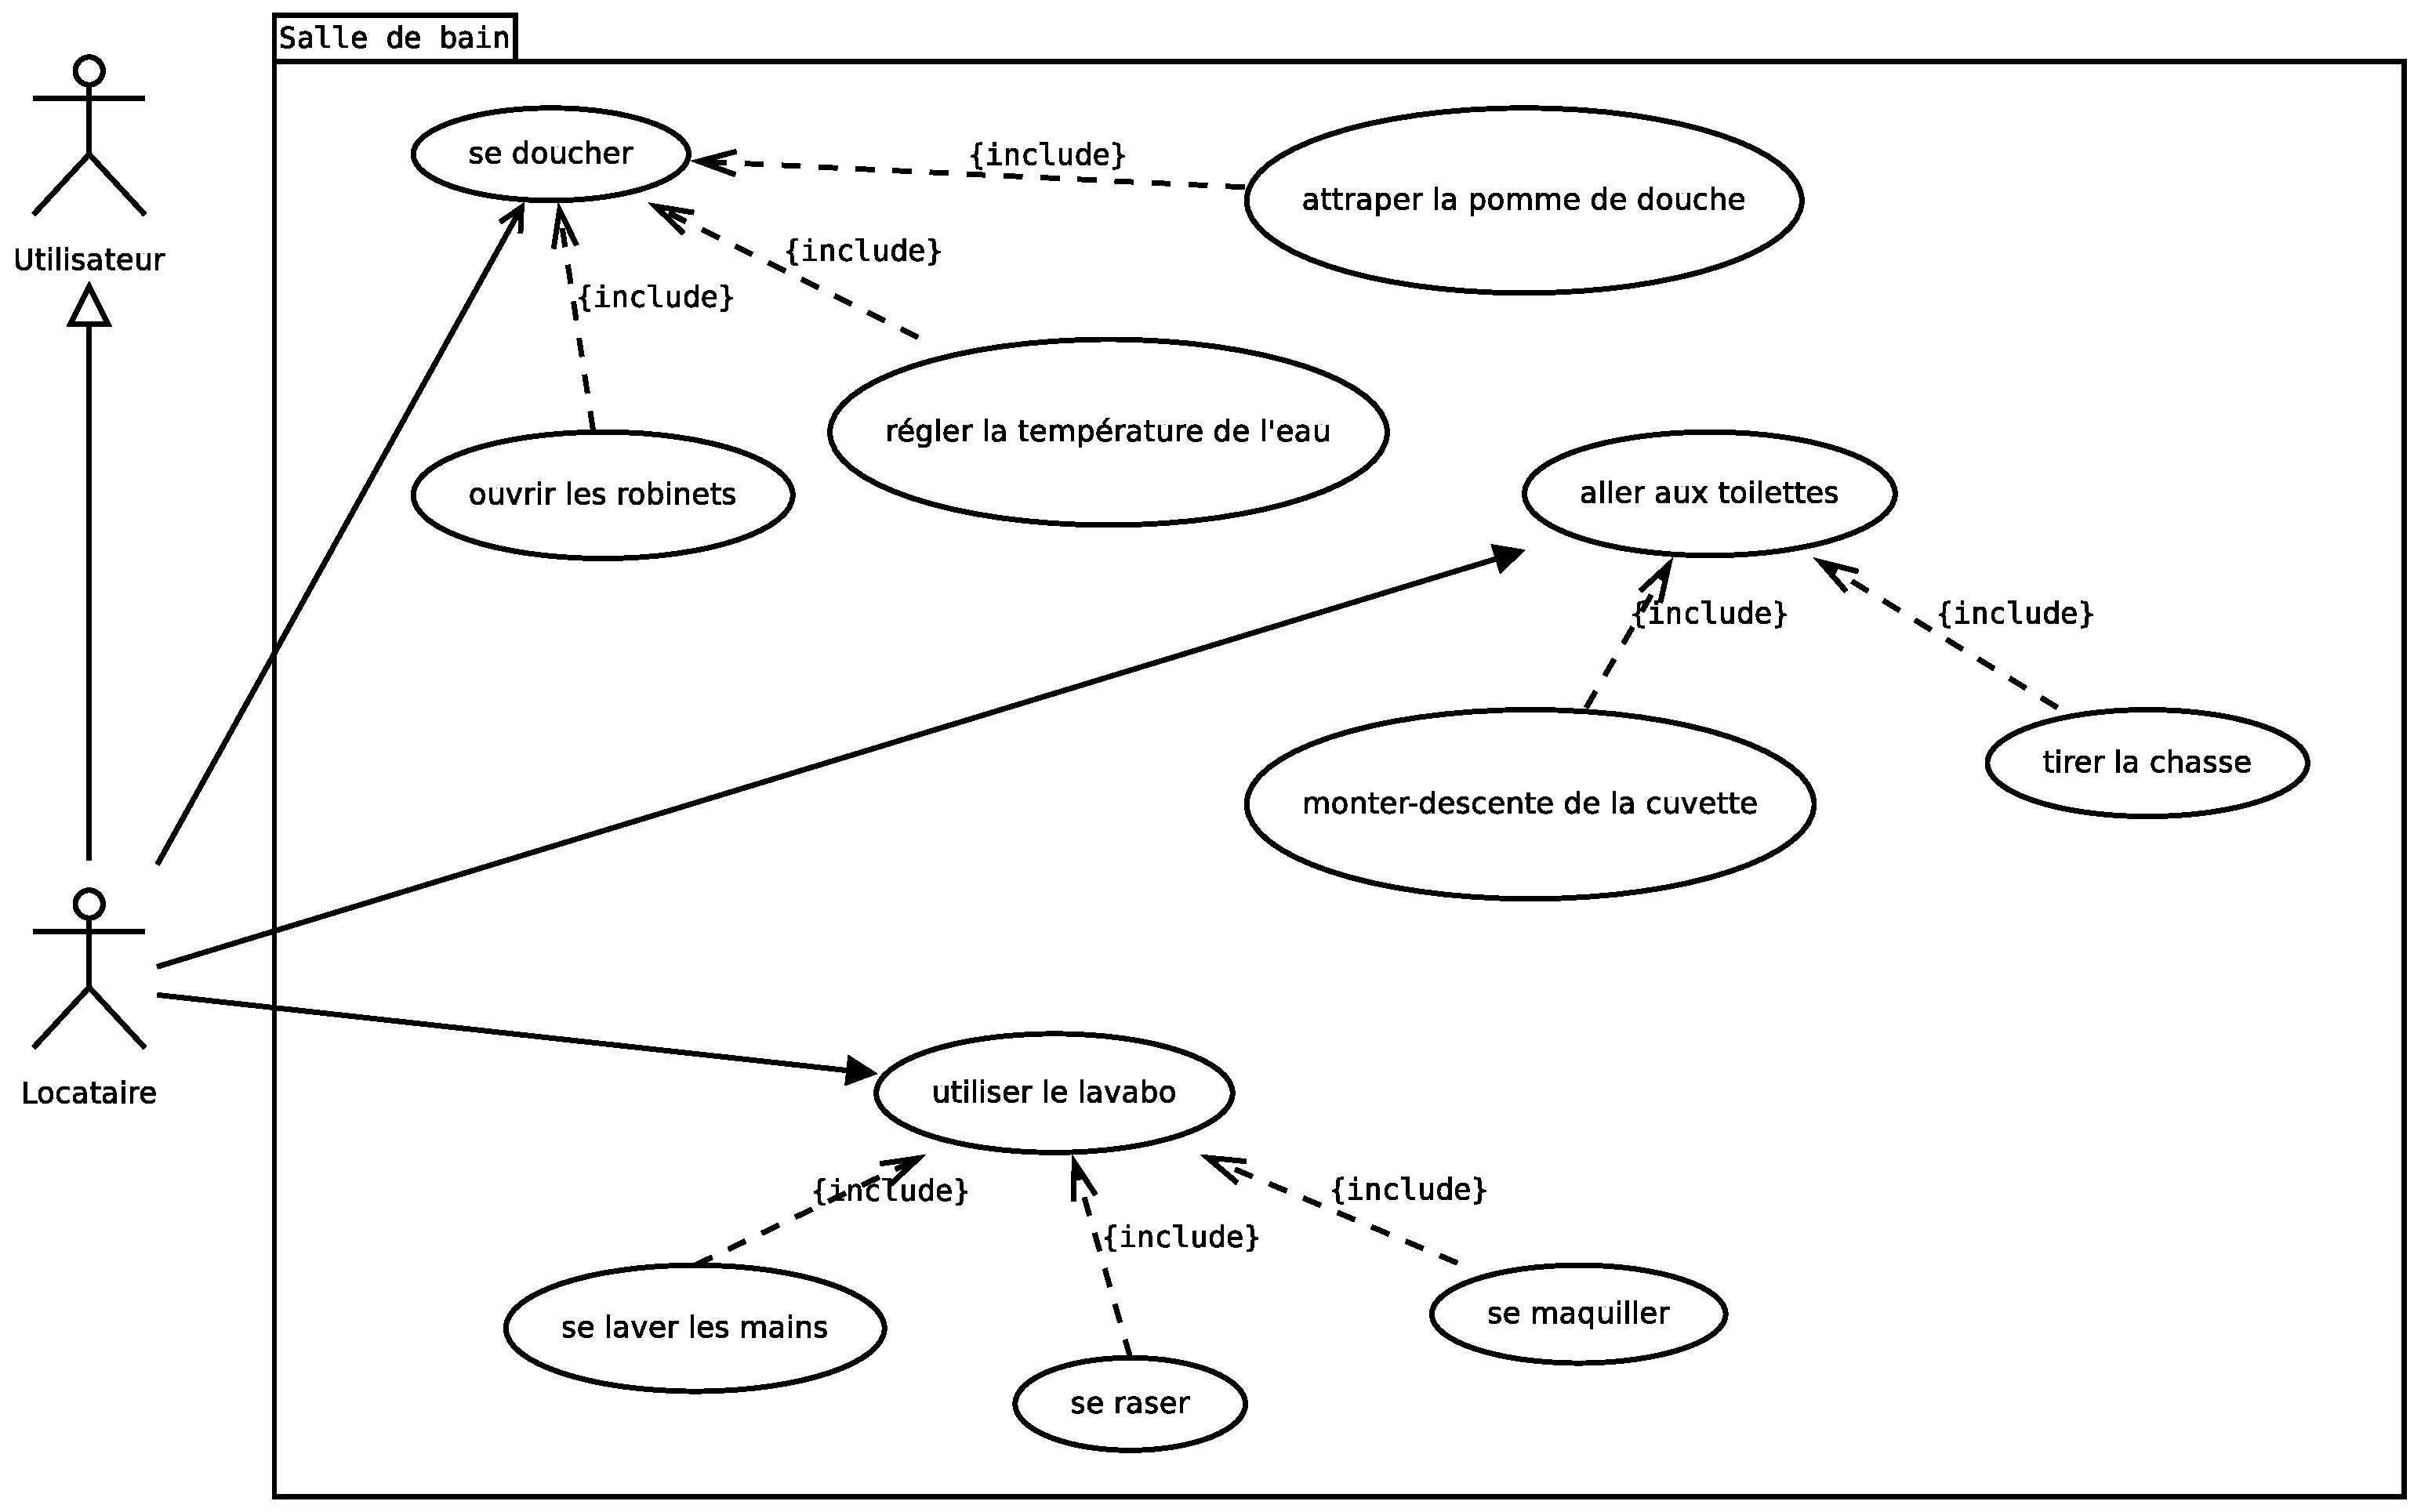
\includegraphics[width=1\linewidth]{diagrams/bathroom/diagramme_cas_utilisation_uc.eps}
	\caption{Diagramme de cas d'utilisation pour un locataire}
	\label{fig:diagramme_cas_utilisation_uc}
\end{figure}
